\section{Architecture}
\label{sec:architecture}

In this Section, we present the \emph{Self-Adaptive Middleware} called \emph{Tekio}.  The platform transforms legacy modules in a processing chain to a self-adaptive one. Tekio is a component centric architecture implemented in OSGi, that provides possibility to replace any of its components at runtime and maintain a clear separation of concerns. At this moment the system is capable of self-configuring and self-optimizing based on QoS feedback. Tekio is built on top of layers as shown in Figure \ref{fig:tekioArch} (a). The lowest software layer is that of OSGi including the Java Virtual Machine. The OSGi layer is primarily responsible for execution of the system using the publish-subscribe paradigm for service oriented architecture. The legacy libraries are called from within domain-specific OSGi components in the second layer. The Java Native Access library is used to access the native library. Finally, Tekio's self-adaptation components (see Section \ref{sec:sec:selfTekio}) manage these domain-specific OSGi components (see \ref{sec:sec:chainTekio}). 

% Put the images side by side.


\begin{figure}
%	[H] \centering 
	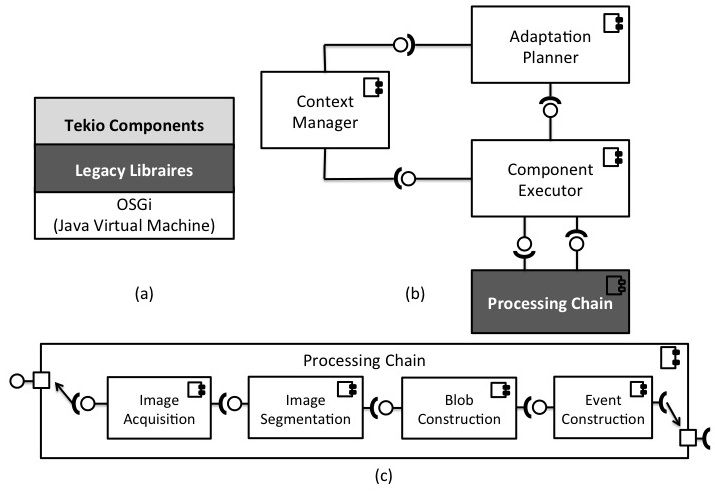
\includegraphics[scale=0.3]{images/architecture.jpg}
	 \caption{Tekio (a) Software Layers (b) Generic Architecture (b) Domain-specific Architecture}
	 \label{fig:tekioArch} 
\end{figure}

\subsection{Tekio Self-adaptation Components} 
\label{sec:sec:selfTekio}

Tekio's self-adaptation is provided by three components as shown in Figure \ref{fig:tekioArch} (b):  (1) The Context Manager that monitors and analyzes context events to know when to request a change in processing chain configuration (2) The Adaptation Planner that produces a change plan and (3) The Executor component that (re)configures the processing chain  and executes it. The new processing chain itself can produce new feedback contextual events. The methodology is based on  the Monitor, Analyze, Plan, Execute, Knowledge (MAPE-K) conceived by IBM in \cite{}. At this moment the system is capable of self-configuring and self-optimizing based on QoS feedback and context awareness. 

Tekio is able to provide four different adaptations types: (a)Parameter Adaptation of any of the running components, (b) Component Adaptation to replace a component at runtime for another that provides a similar task, (c) Context Event Adaptation, depending on events from the  processing chain the system analyzes how to adapt and request a new adaptation, and (d) QoS Adaptation on which the system is able to maintain a minimum level of quality of service. 

\subsection{Processing Chain}
\label{sec:sec:chainTekio}

A processing chain as shown in Figure \ref{fig:tekioArch} (c)  is the current configuration of domains-specific components managed by Tekio. We implement a self-adaptive vision system using Tekio. The domain-specific/vision OSGi components in the processing chain call algorithms implemented in the open-source computer vision library OpenCV(Open Source Computer Vision) 2.1. This library is written in C and C++, as many other computer vision libraries for performance benefits. 

We achieve the link between OSGi and legacy libraries using the Java library, Java Native Access (JNA), that seamlessly calls C/C++ functions with negligible performance loss. 
A similar implementation  JavaCV \cite{http://code.google.com/p/javacv/} uses the native access functionality. Technically,  we pass the memory address of an image to the OpenCV C++ functions. This allows  the OSGi framework to manage the native implementation and its process without compromising its performance and original OpenCV library functionalities. The interfaces of the different algorithms are defined in Java while the implementations of the component is in C++. This improves portability and usability of the vision components with  all other components written in the OSGi framework. Any other OSGi component can execute the functionality of these vision components without worrying about low-level and native implementation detail in C/C++.

The vision system's processing chain consists on four types of algorithms: 1) Image acquisition that provides images from different possible sources such as, cameras, streams or files, 2)Image Segmentation that divides images and extracts important objects, 3) Blob Construction and Object Detection that merges the separate objects  into a group called a blob and then into an object such as a face 4) Event  Construction that converts information at different stages of the vision system to produce either events that are fed back to Tekio or events to final users. Each type of algorithm has several possible implementations that are  different manners or configurations to provide specific tasks. For instance, if we use the Smooth Segmentation and the Find Contours blob construction algorithms the system can detect motion. If the Pyramid Segmentation and the HAAR blob construction algorithms are used the system can detect faces. However, if the last configuration uses FGD Segmentation algorithm instead of the pyramid the system can perform faster FPS but lower result quality.

